\documentclass[11pt]{article}
\usepackage[a4paper,margin=2cm]{geometry}
\usepackage[T1]{fontenc}
\usepackage{amsmath,amssymb}
\usepackage{microtype}
\usepackage{enumitem}
\usepackage[hidelinks]{hyperref}
\usepackage{xcolor}
\usepackage{tikz}
\usetikzlibrary{positioning,arrows.meta,shapes.misc}
\usepackage[htt]{hyphenat}
\tolerance=2000 \emergencystretch=3em \hbadness=2000
\setlength{\parindent}{0pt}\setlength{\parskip}{2.5pt}

\newcommand{\code}[1]{\texttt{#1}}
\setlist{nosep,leftmargin=1.4em}

\title{\vspace{-1.5em}Part II --- Adaptive planning in \texttt{cmbagent\_lg}}
\author{}
\date{}

\begin{document}
\maketitle
\vspace{-3em}

\noindent\textbf{Multi-Agent Systems and Agentic AI --- Part II} \quad written individually by Zixuan Wang (zw499).\\
Studied in full at commit \href{https://github.com/borisbolliet/cmbagent_lg/tree/d7d0592a714e4cc01c97f1b77afdd57a208b18db}{\texttt{d7d0592}}
(\texttt{adaptive-planning} branch), module \href{https://github.com/borisbolliet/cmbagent_lg/tree/d7d0592a714e4cc01c97f1b77afdd57a208b18db/cmbagent_lg/adaptive_planning}{\texttt{cmbagent\_lg/adaptive\_planning}}
(graph, nodes, state, schemas, prompts), which composes the \texttt{planning/} and \texttt{deep\_research/} modules.

\section*{II.1\quad Workflow diagram}

\begin{figure}[h]
\centering
\scalebox{0.84}{%
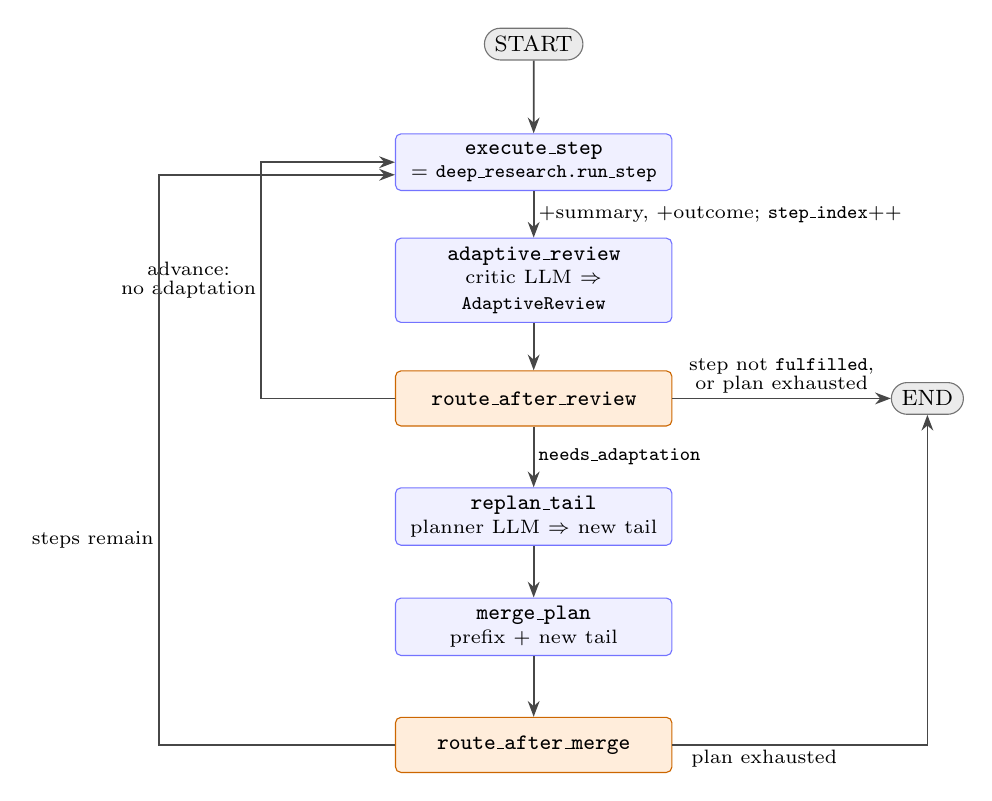
\begin{tikzpicture}[
  >={Stealth[length=2mm,width=1.5mm]}, font=\footnotesize,
  proc/.style={rectangle, rounded corners=2pt, draw=blue!55, fill=blue!6, align=center,
               inner sep=3pt, minimum height=7mm, text width=33mm},
  rt/.style={rectangle, rounded corners=2pt, draw=orange!80!black, fill=orange!14, align=center,
             inner sep=3pt, minimum height=7mm, text width=33mm},
  term/.style={rounded rectangle, draw=black!55, fill=black!8, align=center, inner sep=3pt},
  e/.style={->, semithick, draw=black!72},
  lbl/.style={font=\scriptsize, inner sep=1.5pt},
]
\node[term] (start) at (0,0) {START};
\node[proc] (exec)   at (0,-1.5) {\code{execute\_step}\\[-1pt]{\scriptsize $=$ \code{deep\_research.run\_step}}};
\node[proc] (rev)    at (0,-3.0) {\code{adaptive\_review}\\[-1pt]{\scriptsize critic LLM $\Rightarrow$ \code{AdaptiveReview}}};
\node[rt]   (r1)     at (0,-4.5) {\code{route\_after\_review}};
\node[proc] (replan) at (0,-6.0) {\code{replan\_tail}\\[-1pt]{\scriptsize planner LLM $\Rightarrow$ new tail}};
\node[proc] (merge)  at (0,-7.4) {\code{merge\_plan}\\[-1pt]{\scriptsize prefix $+$ new tail}};
\node[rt]   (r2)     at (0,-8.9) {\code{route\_after\_merge}};
\node[term] (end)    at (5.0,-4.5) {END};

\draw[e] (start) -- (exec);
\draw[e] (exec)  -- (rev)  node[lbl,midway,right]{$+$summary, $+$outcome; \code{step\_index}{+}{+}};
\draw[e] (rev)   -- (r1);
\draw[e] (r1)    -- (replan) node[lbl,midway,right]{\code{needs\_adaptation}};
\draw[e] (replan)-- (merge);
\draw[e] (merge) -- (r2);
\draw[e] (r1.east) -- (end) node[lbl,midway,above,align=center]{step not \code{fulfilled},\\[-1pt] or plan exhausted};
\draw[e] (r2.east) -| (end) node[lbl,pos=0.18,below]{plan exhausted};
% back-edges to execute_step (next step)
\draw[e] (r1.west) -- ++(-1.7,0) |- (exec.west) node[lbl,pos=0.25,left,align=center]{advance:\\[-1pt] no adaptation};
\draw[e] (r2.west) -- ++(-3.0,0) |- ([yshift=-1.6mm]exec.west) node[lbl,pos=0.18,left]{steps remain};
\end{tikzpicture}}
\caption{Adaptive-planning LangGraph graph (\code{adaptive\_planning/graph.py}). Blue $=$ work nodes, orange $=$ conditional
routers; the threaded \code{AdaptivePlanState} carries \code{plan}, \code{step\_index}, \code{step\_summaries}/\code{step\_outcomes},
\code{adaptive\_review}, \code{new\_tail}, \code{adaptive\_history}. \emph{(Excluded from the 2-page limit.)}}
\end{figure}

\noindent\textbf{Walkthrough.} The initial \code{Plan} comes from the bounded propose--critique loop in \code{planning/}; this graph
executes it. \code{execute\_step} (\code{deep\_research}'s \code{run\_step}, reused verbatim) runs the step at \code{step\_index},
appends a summary and a structured outcome \{\code{fulfilled},\dots\}, increments \code{step\_index}, and always passes to
\code{adaptive\_review}.
\emph{Trigger:} \code{adaptive\_review} --- a critic LLM given the overall task, the step's summary$+$outcome, and the unrun steps ---
returns \code{AdaptiveReview(needs\_adaptation, recommendations)}; \code{route\_after\_review} goes to \code{replan\_tail} \emph{iff}
the step was \code{fulfilled}, the plan is not exhausted, \emph{and} \code{needs\_adaptation} --- otherwise it advances or halts at
\code{END}.
\emph{Mutable vs.\ fixed:} only the \emph{tail} \code{plan.sub\_tasks[n\_done:]} changes --- \code{replan\_tail} gets a replacement
tail from the planner LLM (given the completed summaries, current tail, and recommendations) and \code{merge\_plan} sets
\code{plan = completed\_prefix + new\_tail}. The completed prefix, its summaries/outcomes, and \code{step\_index} are frozen, so
executed work is never re-run.
\emph{Termination:} a router returns \code{END} when a step is \emph{not} \code{fulfilled} or \code{step\_index $>$ len(plan)}.
\code{execute\_step} advances \code{step\_index} by one per step and revision never does, so the loop ends only once the replanner
returns a consumable tail --- a \emph{soft} guarantee: it is merely \emph{prompted} to ``keep the tail minimal'', with no revision
counter or length cap, so a non-shrinking replanner is stopped only by LangGraph's default \code{recursion\_limit} (which
\emph{raises} rather than finishing), unlike the initial loop's hard \code{num\_rounds} bound.

\section*{II.2\quad Problems}

\textbf{P1 --- No designed termination or progress guarantee.} \code{step\_index} increases only in \code{execute\_step};
\code{replan\_tail} may return a tail \emph{longer} than the steps it replaces, and \code{merge\_plan} routes straight back into
execution. There is no revision budget, no plan-length cap, and no monotone quantity that must strictly decrease. Closed-loop
control is only well-behaved when the feedback law contracts toward the goal (a termination/Lyapunov argument); a free-text
``keep it minimal'' instruction to an LLM is not such a contraction, and can thrash or diverge. The only hard backstop,
\code{recursion\_limit}, surfaces as an \emph{exception}, not a finished run --- and the safeguard the initial planner relies on
(\code{num\_rounds}) was dropped here.

\textbf{P2 --- Adaptation is disabled exactly when it is most needed.} \code{route\_after\_review} returns \code{END} the instant an
outcome is \code{fulfilled=False} --- and it checks this \emph{before} \code{needs\_adaptation}, so the \code{adaptive\_review} LLM
still runs and its verdict is silently discarded. The loop therefore replans after \emph{successful} steps but \emph{gives up} on a
failed one, with no repair, retry, or route-around. This inverts the purpose of closed-loop control, which exists to reject
disturbances and correct errors: here good news triggers feedback while bad news triggers a halt.

\textbf{P3 --- The replanned tail bypasses the reviewer that gates the initial plan.} \code{planning/} accepts a plan only after a
bounded \code{planner}$\leftrightarrow$\code{plan\_reviewer} propose--critique loop. The adaptive replan has \emph{no} reviewer:
\code{merge\_plan} splices the planner's \code{new\_tail} unchecked. Revisions --- generated mid-run under the pressure of a
surprising result, i.e.\ exactly when error is likeliest --- thus receive \emph{weaker} quality control than the original plan, and
can drift from \code{main\_task} or contradict the frozen prefix with nothing to catch it.

\textbf{P4 --- Myopic feedback at unconditional cost.} \code{adaptive\_review} sees only the \emph{last} step's summary$+$outcome and
the remaining steps --- not the full trajectory or the artifacts produced --- so its decision is greedy (Markov on the last step)
and cross-step drift is invisible; closed-loop control needs full-state feedback, not a single observation. It also fires after
\emph{every} step regardless of need (and the planner on every revision), so token cost and latency scale with plan length with no
gating.

\section*{II.3\quad Proposed improvements}

\textbf{P1 $\to$ bound the loop.} Thread a \code{revision\_budget} (and/or \code{max\_steps}) through \code{AdaptivePlanState},
decrement it in \code{merge\_plan}, and have the routers \emph{finish gracefully} (run out the current tail, then \code{END}) once it
hits zero; optionally reject any \code{new\_tail} that would push the plan past a length cap. \emph{Why:} reinstates a
strictly-decreasing quantity, so termination no longer rests on LLM goodwill. \emph{Trade-off:} a hard cap can truncate a genuinely
expanding task --- so surface ``budget exhausted'' as an explicit, inspectable outcome rather than a silent stop.

\textbf{P2 $\to$ repair on failure instead of halting.} On \code{fulfilled=False}, route to \code{replan\_tail} (or a dedicated
\code{repair} node) with a per-step retry budget, halting only after $K$ failed attempts. \emph{Why:} makes the loop genuinely
closed over errors --- the failure becomes the feedback that drives a re-plan, which is the entire point of adaptive planning.
\emph{Trade-off:} extra execution/LLM cost and a risk of looping on an impossible step, both bounded by the retry budget; needs a
recoverable-vs-fatal flag in the outcome.

\textbf{P3 $\to$ validate the replanned tail.} Before \code{merge\_plan}, pass \code{new\_tail} through the existing \code{planning}
\code{plan\_reviewer} for one critique round against \code{main\_task} and the frozen prefix, regenerating if it diverges.
\emph{Why:} gives revisions the same quality gate as the initial plan, closing the asymmetry in P3. \emph{Trade-off:} one extra
reviewer call (and possibly a planner re-pass) per revision --- bound it to a single round to cap added latency.

\textbf{P4 $\to$ richer, gated feedback.} Give the reviewer the full step history and original goal (global state), and \emph{gate}
the call --- use a cheap model (or skip it) when the outcome shows no downstream impact, escalating to the full critic only on
flagged steps. \emph{Why:} full-state feedback catches multi-step drift; gating removes the per-step tax. \emph{Trade-off:} more
context costs tokens, and gating risks missing a non-obvious adaptation --- so gate conservatively.

\end{document}
